%!TEX root = ../TechnischerEntwurf.tex

\chapter{Analyse der Produktfunktionen}\label{chap:analyse}

Im Folgenden werden die im Pflichtenheft benannten Funktionen näher beschrieben und erkl\"art. Dabei wird davon ausgegangen, dass der User sich in dem Interface befindet, in dem er die erklärte Funktion initiieren kann.

Des Weiteren ist zu erkennen, dass, jedes mal wenn das Back-End nach der Registration oder dem Login aktiv wird, es zuerst einen \glqq checkSession()\grqq -Methodenaufruf startet. Dies ist die Überprüfung des Back-Ends, ob es selbst den User kennt, ob er die gebrauchten Rechte für die Aktion hat und ob die Aktion auch auf die zum User gehörenden Daten ausgeführt wird.

\newpage
\section{Analyse von Funktionalität <F10>: <Nutzer registrieren>}
\label{sequence_f10}
\begin{figure}[htb]
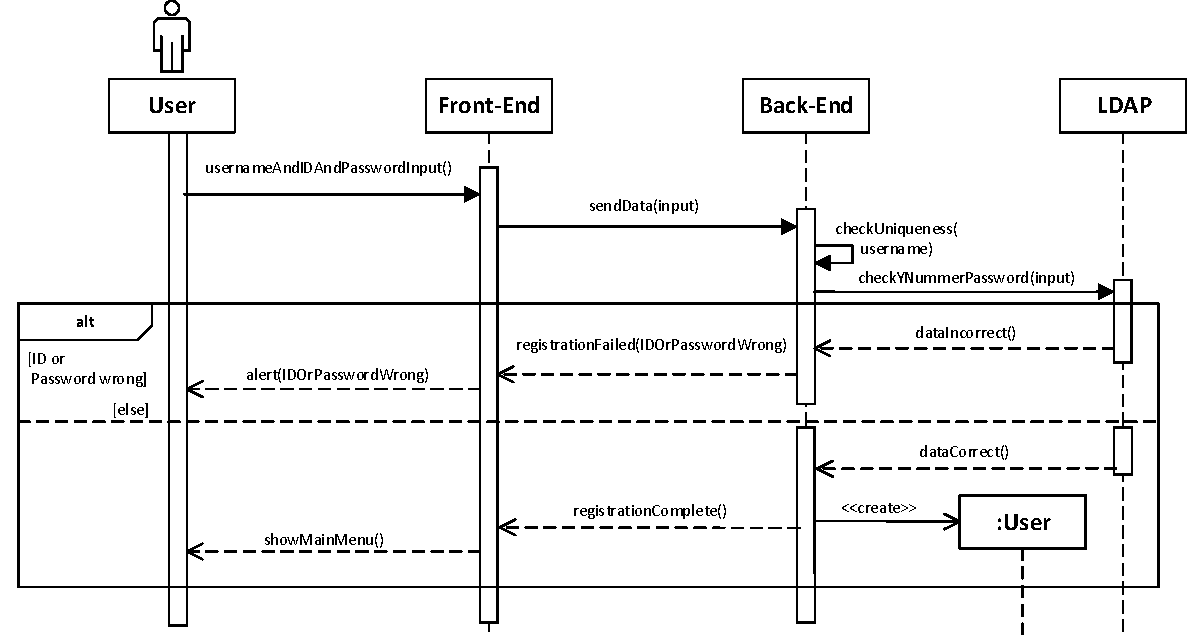
\includegraphics[width=1\textwidth]{figures/sequenz_F10.pdf}
\caption{Sequenzdiagramm zur Registrierung}
\end{figure}

In Diagramm \ref{sequence_f10} wird der Vorgang der Registrierung beschrieben.

Dafür muss der User zuerst einen Username, eine E-Mail-Adresse oder seine y-Nummer (insgesamt ID genannt) und ein Passwort (im Falle einer y-Nummer das zur y-Nummer gehörende Passwort) angeben. Diese Eingaben werden dann an das Back-End übertragen. Hier wird zuerst geprüft ob der Username schon vergeben ist. Sollte das der Fall sein, wird dies dem User mitgeteilt und er muss einen neuen Username angeben.
Wenn der Username noch nicht vergeben war, wird, im Falle dass es sich bei der ID um eine E-Mail-Adresse handelt, geprüft, ob diese schon vorhanden ist. Wenn die ID eine y-Nummer ist, wird diese, inklusive des eingegebenen Passworts, an das \glqq LDAP\grqq ~geschickt und dort überprüft. Sollte der jeweils zutreffende Schritt fehlschlagen, muss der User seine Eingaben ändern, beziehungsweise korrigieren und der Prozess beginnt von vorn.

Sollte der Ablauf erfolgreich abgeschlossen worden sein, erstellt das Back-End ein neues User-Objekt, speichert dies in seiner Datenbank und gibt die Rückmeldung, dass die Registrierung erfolgreich gewesen ist. Der User wird dann in das Hauptmenü weitergeleitet.
%==================================================================

\newpage
\section{Analyse von Funktionalität <F20>: <Nutzer anmelden>}
\begin{figure}[h]
\centering
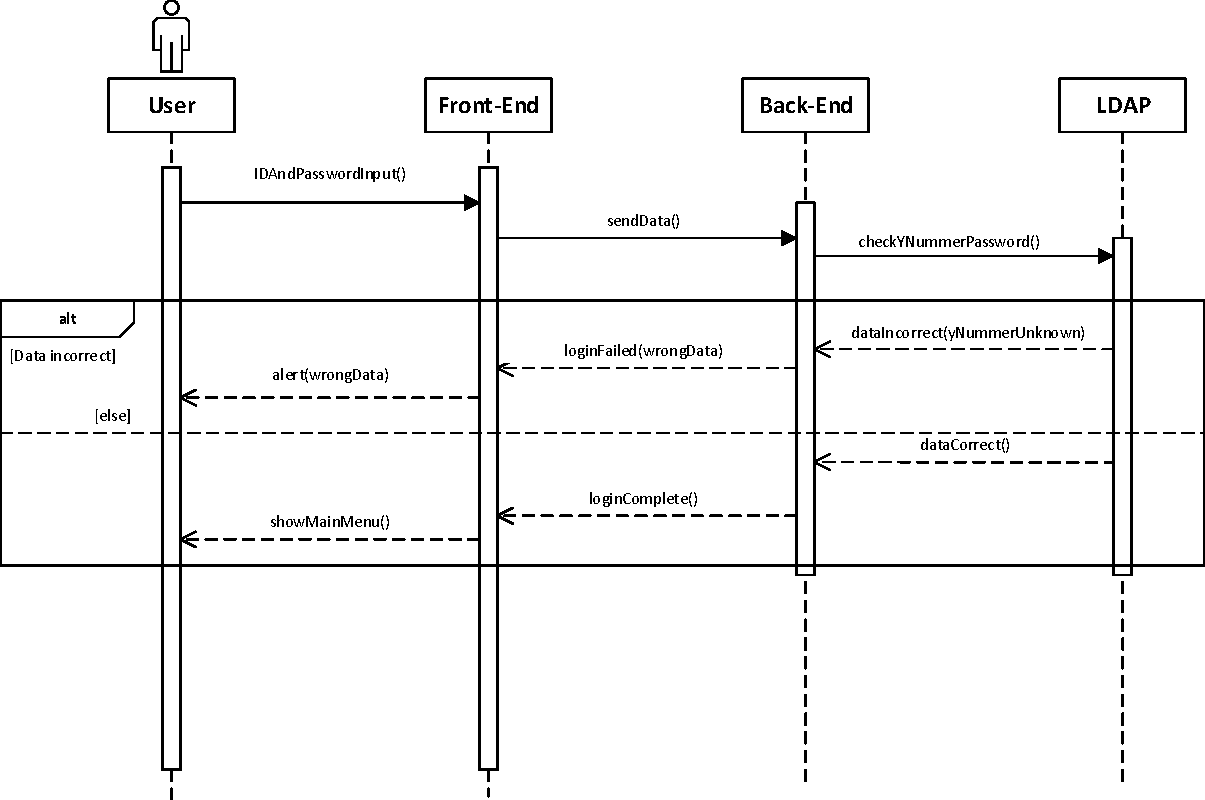
\includegraphics[width=1\textwidth]{figures/sequenz_F20.pdf}
\caption{Sequenzdiagramm zum Login}
\label{sequence_f20}
\end{figure}
Das Diagramm \ref{sequence_f20} beschreibt den Login-Vorgang. 

Hierbei muss der User die von ihm registrierte ID (siehe <F10>) und sein Passwort angeben. Diese werden, je nach Typ der ID, dann entweder mit der eigenen Datenbank verglichen, oder, sollte die ID eine y-Nummer sein, an das \glqq LDAP\grqq ~geschickt und dort überprüft.\\
Sollten die eingegeben Daten nicht korrekt sein, wird dies dem User mitgeteilt und er bekommt die Möglichkeit seine Eingaben zu korrigieren. Sind die Daten korrekt wird der User in das Hauptmenü weitergeleitet.
%==================================================================

\newpage
\section{Analyse von Funktionalität <F30>: <Nutzer abmelden>}
\begin{figure}[h]
\centering
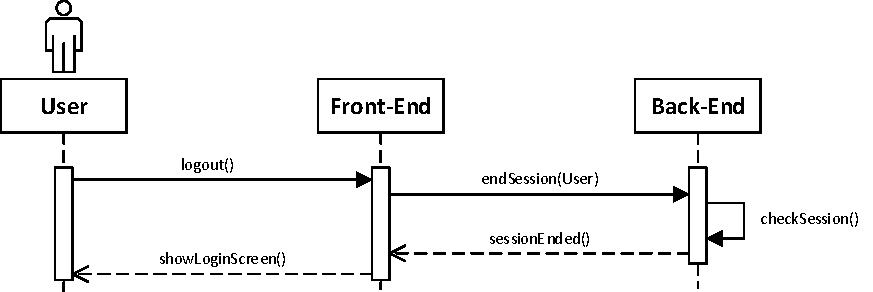
\includegraphics[width=1\textwidth]{figures/sequenz_F30.pdf}
\caption{Sequenzdiagramm zum Login}
\label{sequence_f30}
\end{figure}
Das Diagramm \ref{sequence_f30} beschreibt den Ablauf des Ausloggens.

Entscheidet sich der User dazu sich auszuloggen, wird diese Information an das Back-End gesendet. Dieses beendet die Session des Users. Ist das geschehen wird eine Benachrichtigung an das Front-End gesendet und der User wird zurück zum Login-Screen geleitet.
%==================================================================

\newpage
\section{Analyse von Funktionalität <F40>: <Profil einsehen>}
\begin{figure}[h]
\centering
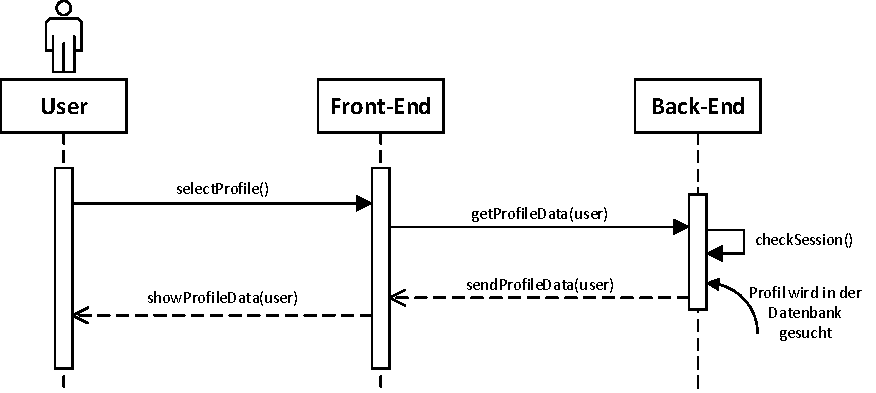
\includegraphics[width=1\textwidth]{figures/sequenz_F40.pdf}
\caption{Sequenzdiagramm zur Darstellung der Profilübersicht}
\label{sequence_f40}
\end{figure}
Das Diagramm  \ref{sequence_f40} zeigt was passiert, wenn man sich das eigene Userprofil anzeigen lassen möchte.

Um das Profil des Users anzuzeigen, werden zuerst die Userdaten vom Back-End angefordert. Das Back-End lädt dann die Profildaten aus den Userdaten und schickt diese zurück an das Front-End. Dort werden sie, für den User einsehbar, im Profil-Interface angezeigt.

%==================================================================

\newpage
\section{Analyse von Funktionalität <F60>: <Passwort ändern>}
\begin{figure}[h]
\centering
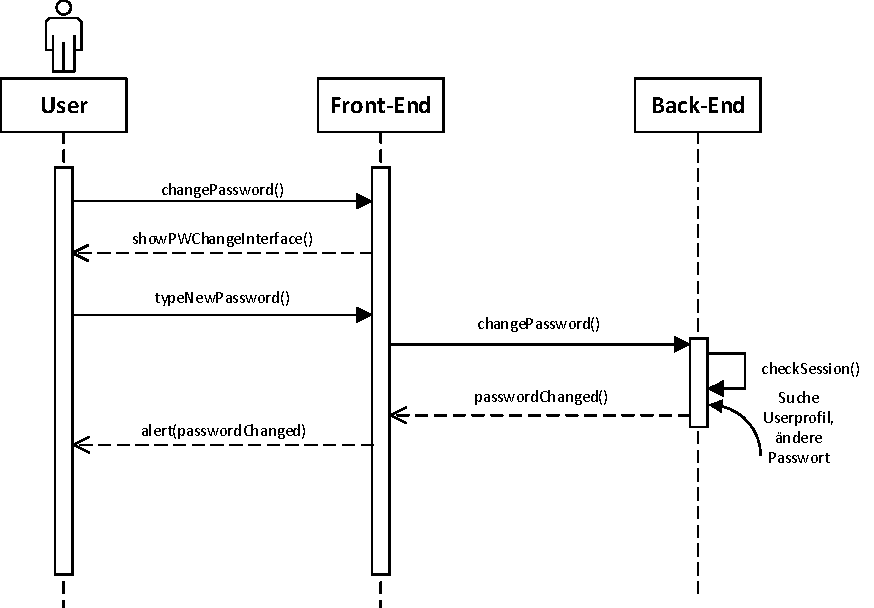
\includegraphics[width=1\textwidth]{figures/sequenz_F60.pdf}
\caption{Sequenzdiagramm zum Ändern des Passworts}
\label{sequence_f60}
\end{figure}
Das Diagramm \ref{sequence_f60} beschreibt das Ändern des Passwortes.

Das Ändern des Passwortes steht nur nicht-studentischen Nutzern zur Verfügung.
Entscheidet sich der Nutzer, sein Passwort zu ändern, kann er dies mit einem Klick auf den \glqq Change Password \grqq -Button tun. Zuerst muss er sein altes Passwort eingeben und im Anschluss kann er ein neues Password erstellen. Dies muss danach noch einmal bestätigt werden und wenn alles erfolgreich war, wird das geänderte Passwort an das Back-End geschickt und dort in den Nutzerdaten vermerkt. Sollte während des Vorgangs ein Fehler auftreten, bleibt das alte Passwort bestehen und der User wird darüber in Kenntnis gesetzt.
%==================================================================

\newpage
\section{Analyse von Funktionalität <F70>: <Avatar ändern>} 
\begin{figure}[h]
\centering
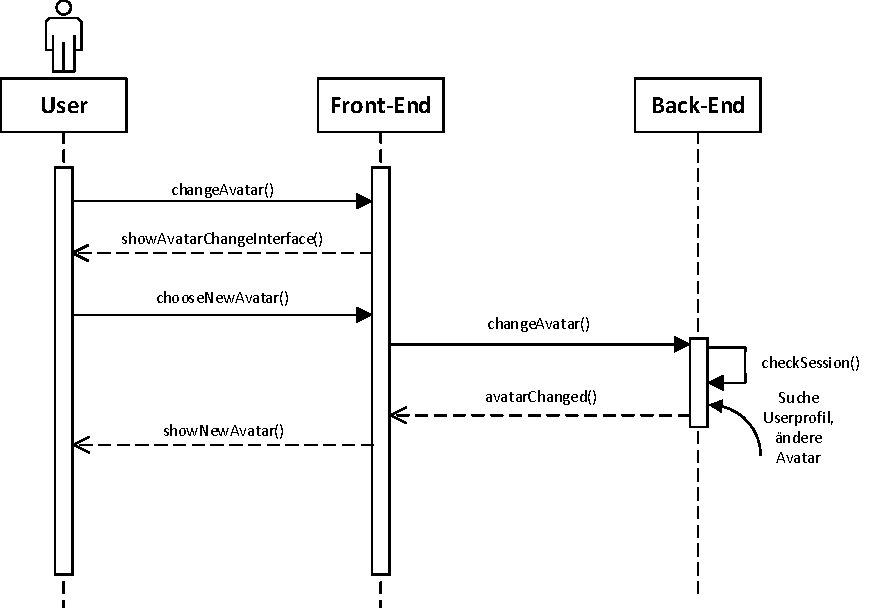
\includegraphics[width=1\textwidth]{figures/sequenz_F70.pdf}
\caption{Sequenzdiagramm zum Ändern des Avatars}
\label{sequence_f70}
\end{figure}
Das Diagramm \ref{sequence_f70} beschreibt das Ändern des Avatars.

Klickt der User auf den \glqq Change Avatar \grqq -Button, werden ihm alle seine verfügbaren Avatare angezeigt und er kann sich für einen entscheiden. Hat er dies getan wird die Änderung der Einstellung vermerkt, ans Back-End geschickt, dort gespeichert und dann, wieder zurück im Front-End, aktualisiert angezeigt.
%==================================================================

\newpage
\section{Analyse von Funktionalität <F80>: <Benutzer löschen>} 
\begin{figure}[h]
\centering
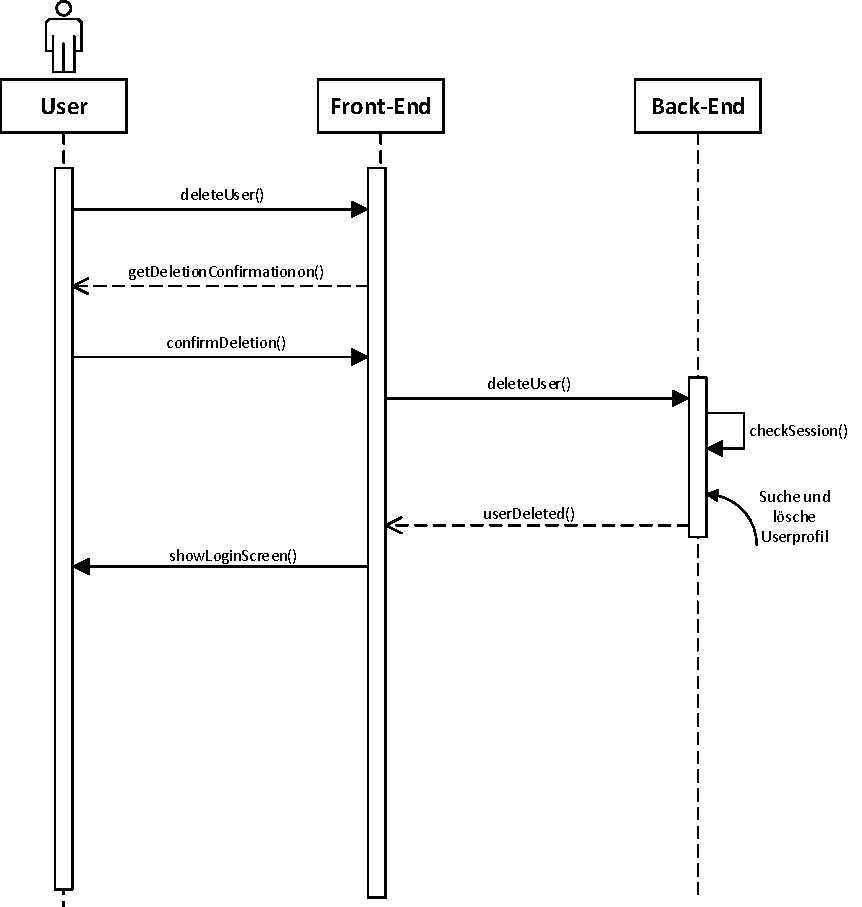
\includegraphics[width=0.9\textwidth]{figures/sequenz_F80.pdf}
\caption{Sequenzdiagramm zum Löschen des Benutzers}
\label{sequence_f80}
\end{figure}
Diagramm \ref{sequence_f80} zeigt, was passiert, wenn der User seinen Account löschen möchte.
Möchte der User sein Profil löschen, kann er dies im Settings-Interface tun, welches dementsprechend erst geladen werden muss. Wenn der User nun den \glqq Delete User\grqq -Button drückt, wird er erst noch einmal gefragt, ob er sein Profil wirklich löschen möchte. Beantwortet der User dies positiv, geht eine Mitteilung an das Back-End, wo das Profil gelöscht wird. Der User wird dann auf den Login-Screen geleitet, wo es ihm frei steht, sich wieder zu registrieren.
%==================================================================

\newpage
\section{Analyse von Funktionalität <F90>: <Audioeinstellungen bearbeiten>}
\begin{figure}[h]
\centering
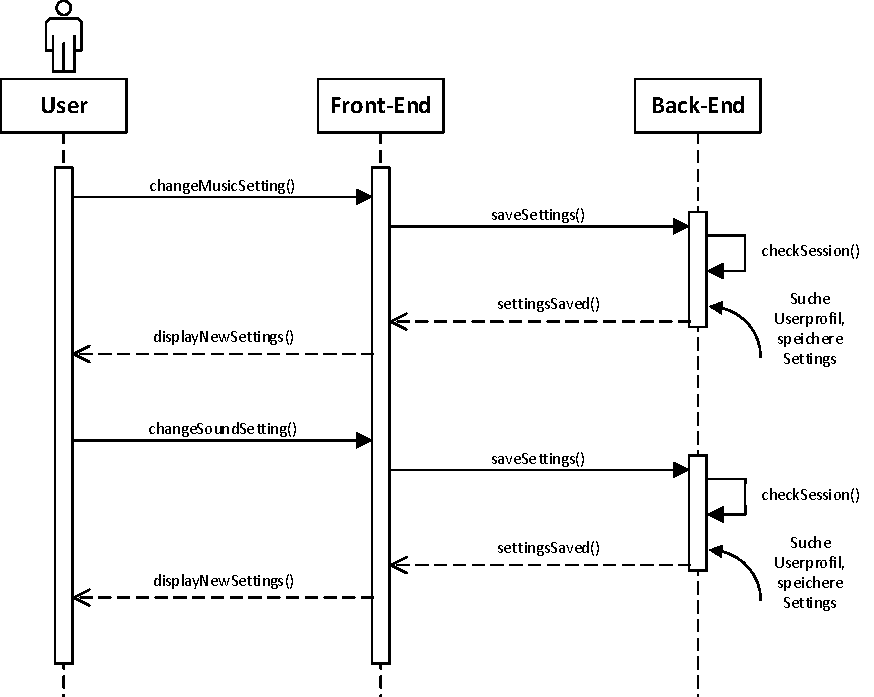
\includegraphics[width=0.9\textwidth]{figures/sequenz_F90.pdf}
\caption{Sequenzdiagramm zum Ändern der Audioeinstellungen}
\label{sequence_f90}
\end{figure}
Diagramm \ref{sequence_f90} zeigt, was passiert, wenn der User seine Audio-Optionen ändert.

Zum Ändern der Audiofunktionen stehen Knöpfe bereit, die sowohl die Hintergrundmusik (\glqq Music\grqq) als auch die Soundeffekte, wie Sprungsounds und Klicksounds,  aus-  beziehungsweise einstellen. Jegliche \"Anderung wird sofort ans Back-End gesendet, dort gespeichert und dann im Profil aktualisiert.
%==================================================================

\newpage
\section{Analyse von Funktionalität <F100>: <Spielstand zurücksetzen>}
\begin{figure}[h]
\centering
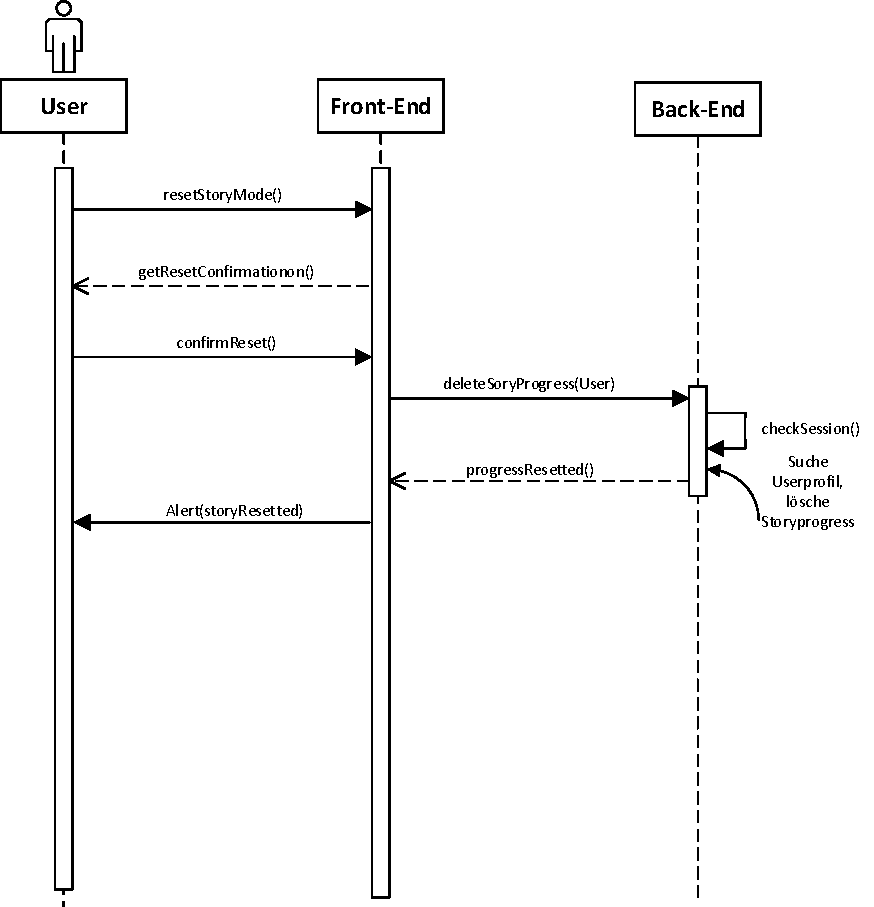
\includegraphics[width=0.9\textwidth]{figures/sequenz_F100.pdf}
\caption{Sequenzdiagramm zum Zurücksetzen des Spielstands}
\label{sequence_f100}
\end{figure}
Diagramm \ref{sequence_f100} beschreibt das Zurücksetzen des Storyfortschritts.

Der User kann per Knopfdruck seinen Story-Fortschritt zurücksetzen. Tut er dies, muss er vorher noch einmal seine Zustimmung zum Löschvorgang geben. Ist auch dies geschehen, wird die Anweisung zum Löschen des Storyfortschritts des Users an das Back-End geschickt und dort ausgeführt.
%==================================================================

\newpage
\section{Analyse von Funktionalität <F110>: <Tutorial spielen>}
\begin{figure}[h]
\centering
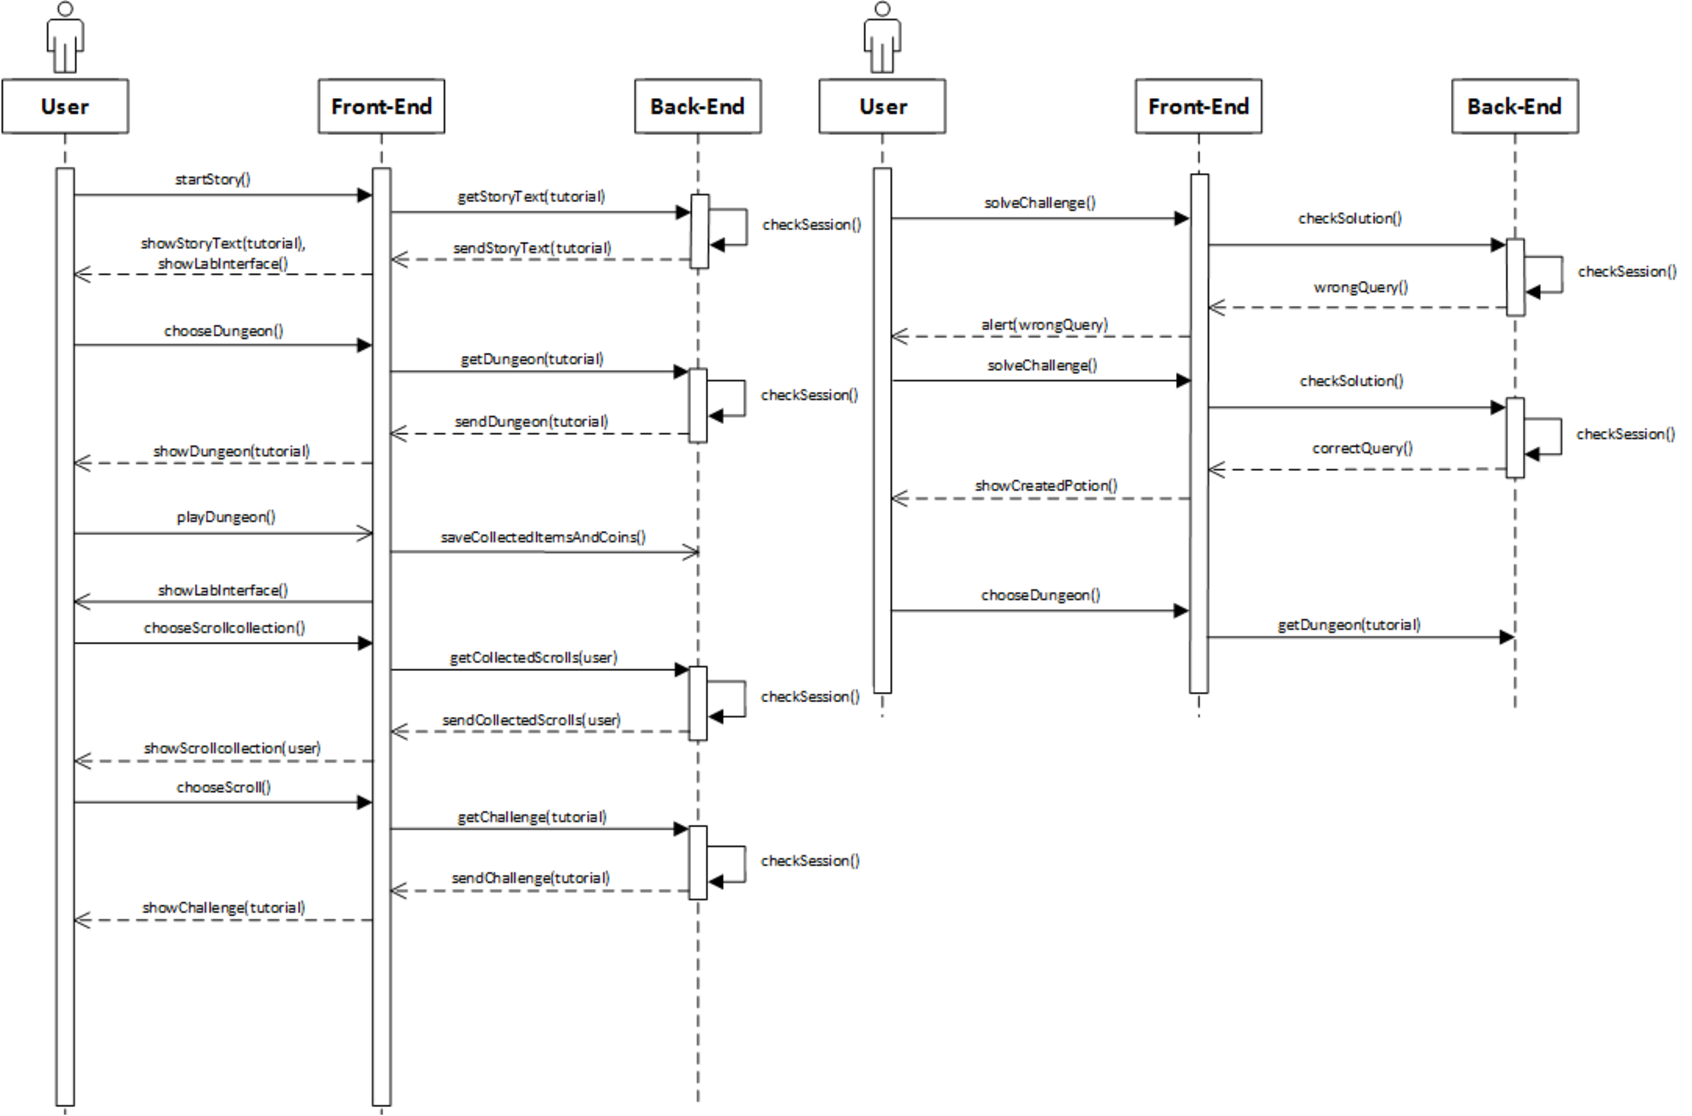
\includegraphics[width=1.0\textwidth]{figures/sequenz_F110.pdf}
\caption{Sequenzdiagramm für das Tutorial}
\label{sequence_f110}
\end{figure}
Diagramm \ref{sequence_f110} zeigt den Ablauf im Tutorial.

Wird das Tutorial gestartet, werden zuerst alle Tutorial-Texte vom Back-End angefordert. Diese werden dann, wenn benötigt, dem User angezeigt. Zuerst wird der User in den Dungeon geleitet. Dazu werden die Leveldaten vom Back-End geladen, sodass der User den Dungeon betreten und spielen kann. Hierbei kann er Schriftrollen (\glqq Scrolls\grqq) und Münzen (\glqq Lofi-Coins\grqq) einsammeln, was jeweils sofort ans Back-End gesendet und dort im Story-Progress bzw. in den Profildaten gespeichert wird.
Scheitert der User an einer Hürde im Dungeon, bekommt er zuerst einen Game-Over-Screen angezeigt, auf dem zu sehen ist, was er eingesammelt hat und wird dann zur\"uck in den Labor-Screen geleitet.
Dort wird er per Tutorial-Text zur Scrollcollection geleitet, um sich dort für ein Trank-Rezept zu entscheiden. Ist dies getan, wird aus dem Back-End eine für das Rezept passende Aufgabe angefordert und dem User angezeigt. Für diese Aufgabe hat der User keine Versuchsbegrenzung. Die Eingaben des Users werden dabei immer an das Back-End gesendet und dort kontrolliert. Hat der User die Aufgabe richtig gelöst, erhält er eine Potion und kann diese danach im Dungeon verwenden.
%==================================================================

\newpage
\section{Analyse von Funktionalität <F120>: <Story spielen>}
\begin{figure}[h]
\centering
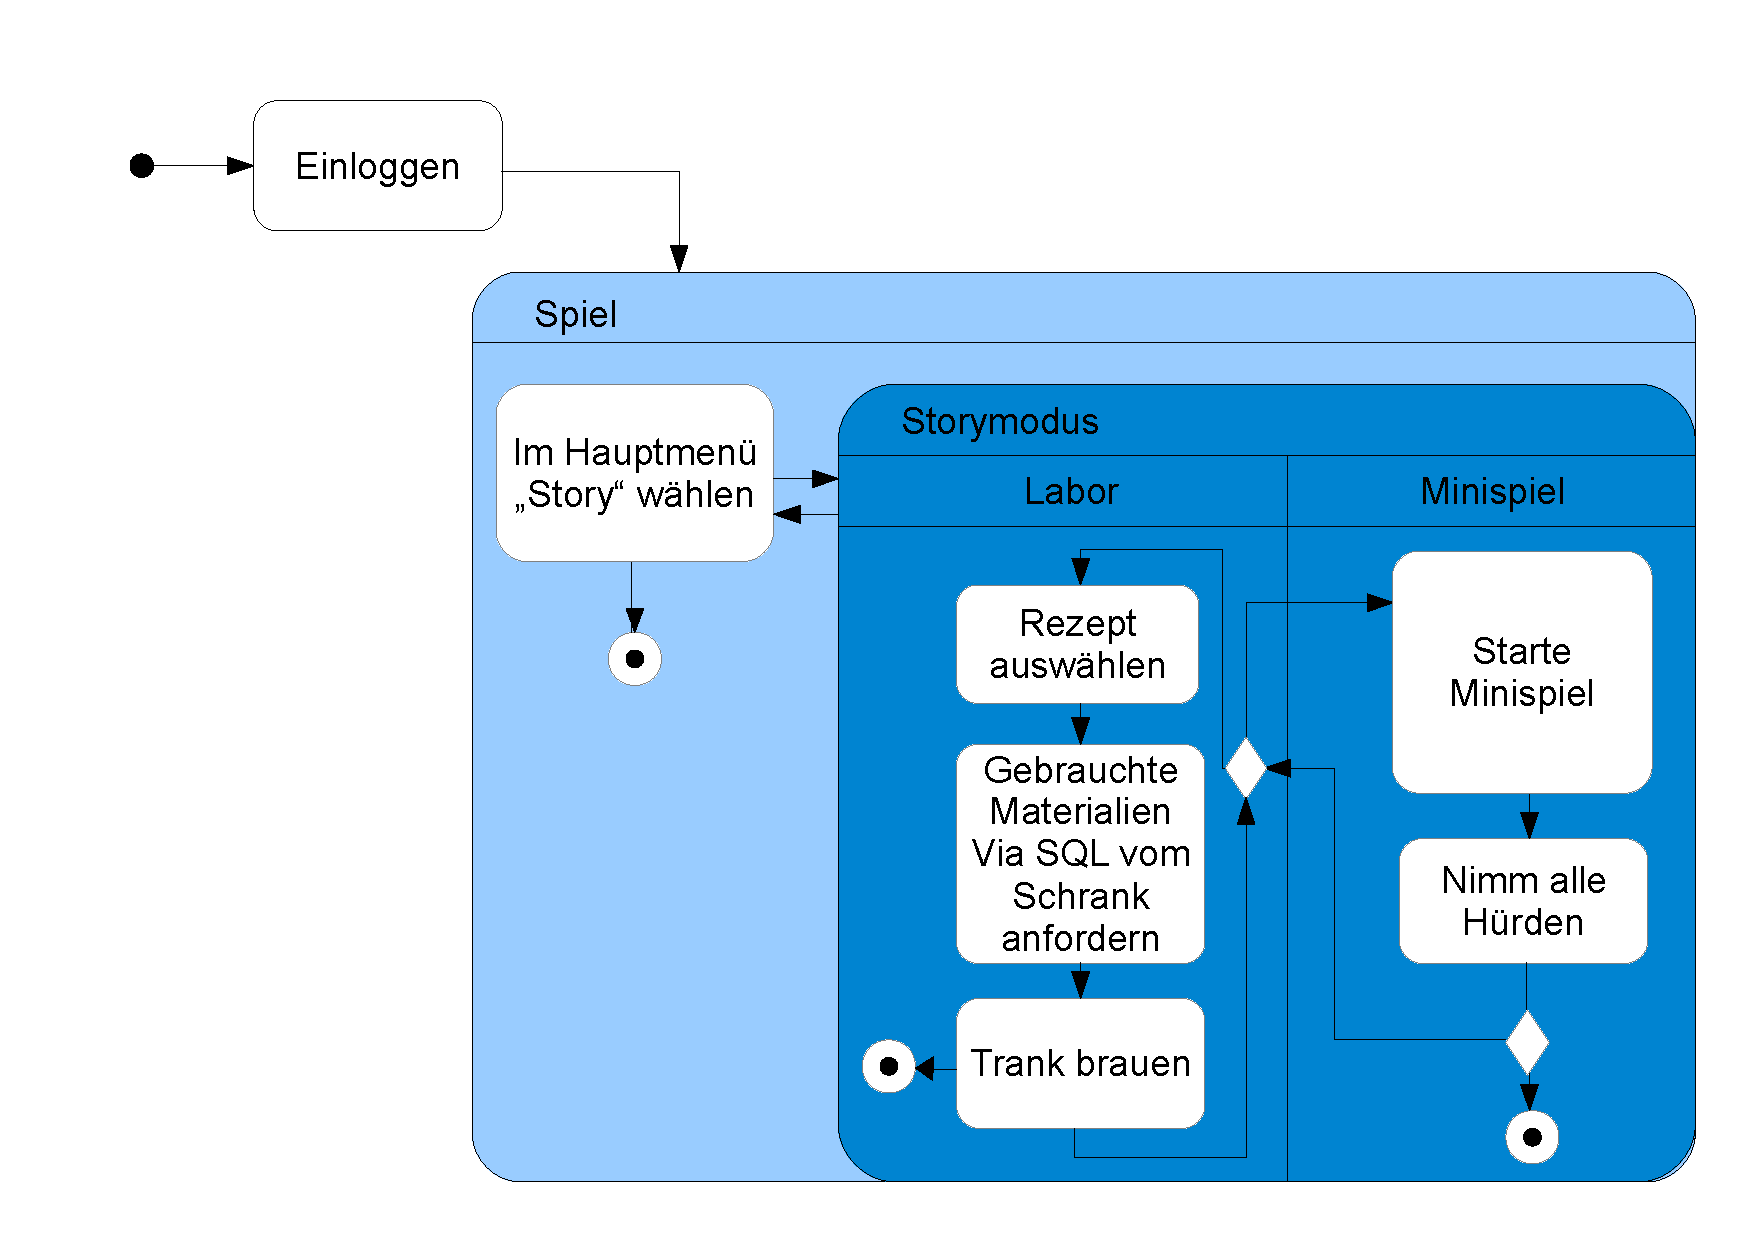
\includegraphics[width=0.9\textwidth]{figures/Aktivitaetsdiagramm.pdf}
\caption{Aktivitätsdiagramm für den Story Mode}
\label{sequence_f120}
\end{figure}
Der Story-Mode besteht zu sich abwechselnden Teilen aus SQL-Trainer und Minispiel. Um dies  besser zu zeigen, ist in Abbildung \ref{sequence_f120} das Aktivitätsdiagramm für den Story Mode aus dem Pflichtenheft abgebildet.\\
Darin ist zu sehen, dass man sich im Labor einen oder mehrere Tränke brauen kann (SQL-Trainer-Anteil), um diese dann im Dungeon zu verwenden (Minispiel-Anteil).
Um die beiden Teile für sich besser beschreiben zu können, sind diese in den folgenden zwei Funktionen separat aufgeführt.
%==================================================================

\newpage
\section{Analyse von Funktionalität <F130>: <SQL-Trainer spielen>}
\begin{figure}[h]
\centering
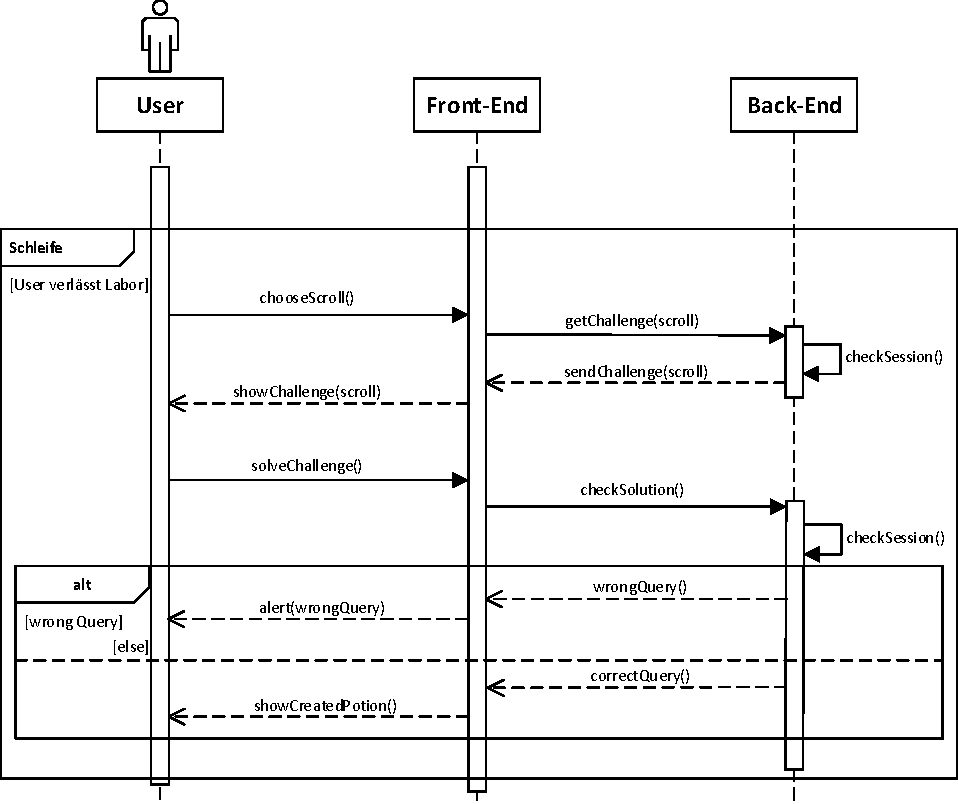
\includegraphics[width=0.9\textwidth]{figures/sequenz_F130.pdf}
\caption{Sequenzdiagramm für den SQL-Trainer}
\label{sequence_f130}
\end{figure}

Der SQL-Trainer ist Teil der drei Spielmodi (Story, Trivia, Homework) und wird einmal (wie er im Trivia-Mode verwendet wird) erklärt. Die leichten Abweichungen der anderen Spielmodi werden im Anschluss erwähnt. Diese benötigen wenig bis gar keine weitere Erklärung, da sie nur einen oberflächlichen Unterschied machen.
Zuerst werden dem User f\"unf Schwierigkeitsgrade angezeigt, aus denen er wählen kann. Hat er sich für einen Schwierigkeitsgrad entschieden, wird dies dem Back-End mitgeteilt, welches daraufhin eine, dem gewählten Schwierigkeitsgrad entsprechende, Aufgabe bereitstellt. Diese kann dann vom User gelöst werden. Die Eingaben werden dabei immer an das Back-End geschickt und dort auf Richtigkeit geprüft. 
Ist die Prüfung positiv verlaufen, wird der User wieder zur Schwierigkeitsgrad-Auswahl weitergeleitet.\\
\newpage
Abweichungen zum Story-Mode:\\
Es werden keine Schwierigkeitsgrade angezeigt, sondern schon eingesammelte Rezepte für Tränke. Diese beinhalten in ihrer Definition schon die Schwierigkeitsgrade für die daraus hervorgehenden Aufgaben.


Abweichungen zum Homework-Mode:\\
Beim Homework-Mode wird die Auswahl des Schwierigkeitsgrades in jeglicher Form übersprungen und der Aufgabentext wird direkt angezeigt.  
%==================================================================

\newpage
\section{Analyse von Funktionalität <F140>: <Minispiel spielen>}
\begin{figure}[h]
\centering
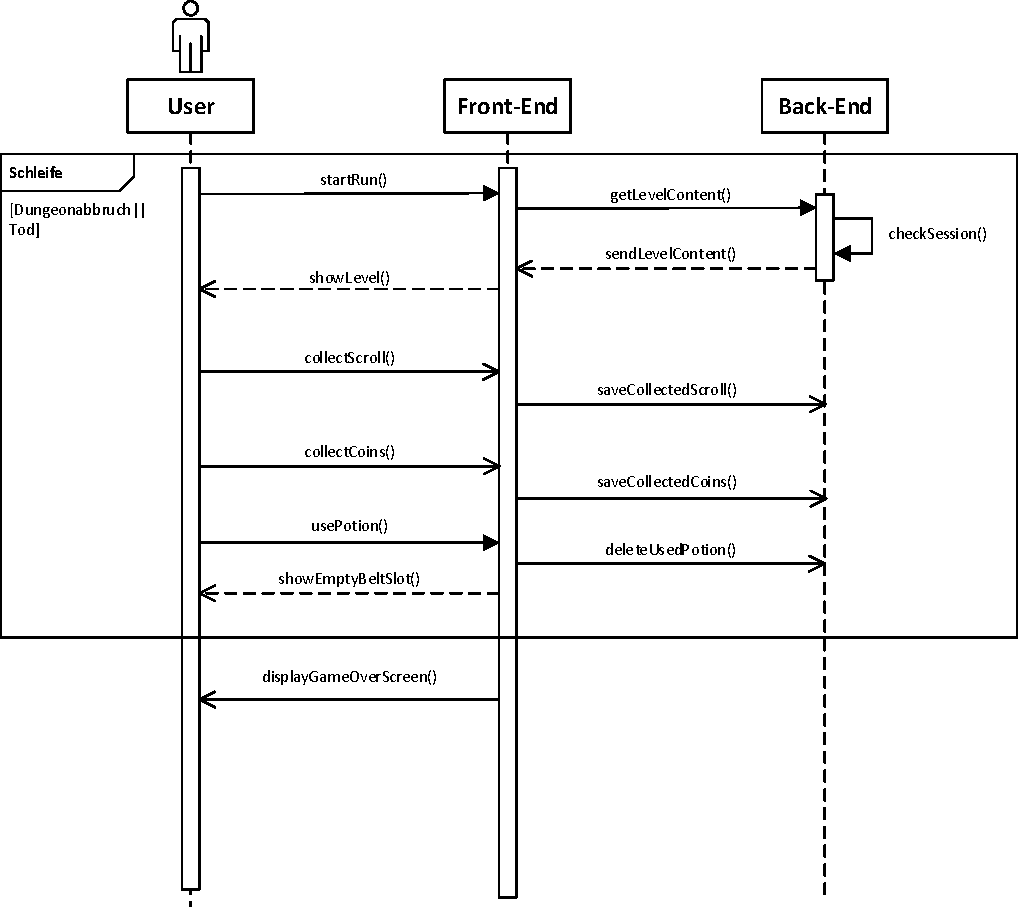
\includegraphics[width=0.9\textwidth]{figures/sequenz_F140.pdf}
\caption{Sequenzdiagramm für das Minigame}
\label{sequence_f140}
\end{figure}
Die Abbildung \ref{sequence_f140} zeigt die Abläufe im Dungeon.

Im Minispiel bewegt sich die Figur stetig nach rechts. Der User kann springen, wodurch er verschiedene Hindernisse überwinden kann. Des Weiteren kann der User Lofi-Coins und Scrolls einsammeln. Dies wird sofort im Back-End vermerkt und im Spielerprofil und im Storyprogress gespeichert. Dem User ist zudem möglich, vorher erstellte Potions zu verwenden, um deren Effekte zur Überwindung von Hindernissen zu nutzen.

%==================================================================

\section{Analyse von Funktionalität <F150>: <Hausaufgaben bearbeiten>}
Die Bearbeitung von Hausaufgaben funktioniert wie das Nutzen des SQL-Trainers. Genauere Erklärungen sind unter (F130) zu finden. Von der dortigen Beschreibung gibt es allerdings folgende Abweichungen: 

Bei den Hausaufgaben handelt es sich um Aufgabenpakete, welche durch die Lehrenden des Moduls RDB1 erstellt werden und den Studenten, die das Modul belegen, zugewiesen werden. Alle anderen Nutzer der Anwendung haben keinen Zugriff auf diese Aufgaben. Die gestellten Aufgabenpakete werden dann als Teil der Studienleistung betrachtet, welche erfüllt werden muss, um RDB1 zu bestehen. Daher sind die Aufgaben nur in den vorgesehenen Bearbeitungszeiträumen erreichbar und zur Bearbeitung freigegeben. 
%==================================================================

\section{Analyse von Funktionalität <F160>: <Ranglisten einsehen>}
\begin{figure}[h]
\centering
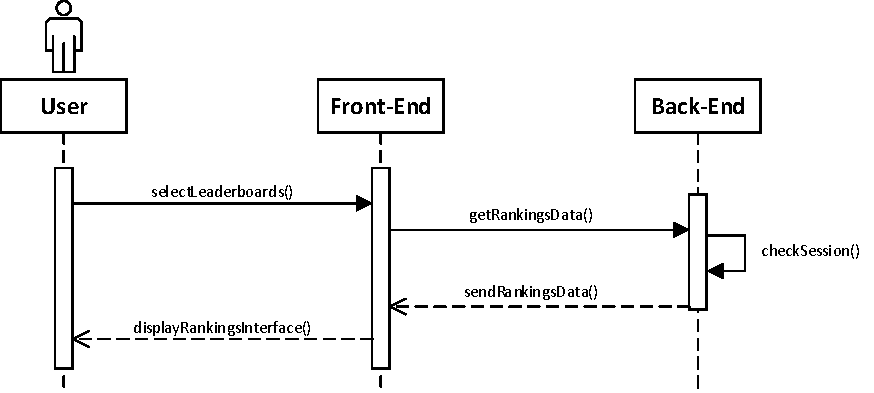
\includegraphics[width=0.9\textwidth]{figures/sequenz_F160.pdf}
\caption{Sequenzdiagramm für die Ranglisten}
\label{sequence_f160}
\end{figure}
In Abbildung \ref{sequence_f160} wir das Anzeigen der Ranglisten dargestellt.

Möchte der User die Ranglisten einsehen, wird eine Anfrage an das Back-End gesendet. Das Back-End stellt dann die Daten für die Ranglisten zusammen und sendet diese zurück an das Front-End, wo diese dann für den User einsehbar präsentiert werden.
%==================================================================

\newpage
\section{Analyse von Funktionalität <F170>: <Spieler suchen>}
\begin{figure}[h]
\centering
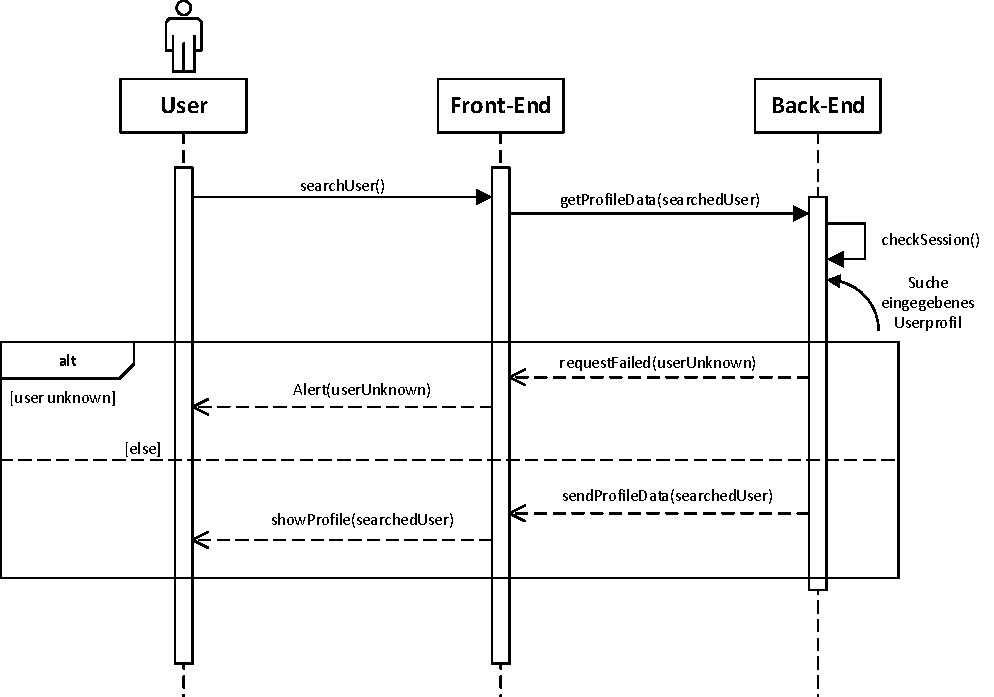
\includegraphics[width=0.9\textwidth]{figures/sequenz_F170.pdf}
\caption{Sequenzdiagramm zum Suchen eines anderen Users}
\label{sequence_f170}
\end{figure}
Im Diagramm \ref{sequence_f170} ist zu sehen, wie man nach einem anderen User suchen kann.

Um einen anderen User zu suchen, wird ein Eingabefeld bereitgestellt. Der dort eingegebene Name wird an das Back-End weitergeleitet, dort in der Userdatenbank gesucht und wenn er existiert, wird dessen Profil aus der Datenbank geladen und dem suchenden User angezeigt. Ist der Name in der Datenbank nicht zu finden, wird dies dem suchenden User mitgeteilt.

Der Zweck der Suche ist es, dass die User die Profile anderer Spieler einsehen können, um sich mit diesen vergleichen zu können. Dies kann aus Gründen des Wettbewerbs untereinander oder einfach aus dem Interesse am Fortschritt von bekannten Usern geschehen. Somit bietet die Funktion den Usern eine simple Möglichkeit sich mit anderen Spielern zu vergleichen.
%================================================================== 

\newpage
\section{Analyse von Funktionalität <F180>: <Hausaufgabenergebnisse einsehen>}
\begin{figure}[h]
\centering
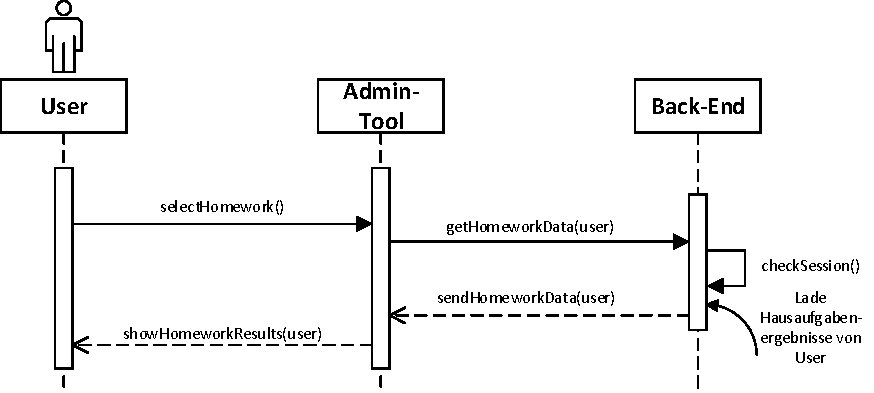
\includegraphics[width=0.9\textwidth]{figures/sequenz_F180.pdf}
\caption{Sequenzdiagramm zum einsehen der eigenen Hausaufgabenergebnisse}
\label{sequence_f180}
\end{figure}
Abbildung \ref{sequence_f180} beschreibt das Anzeigen der Hausaufgabenergebnisse.

Nach dem Einloggen in das Admintool werden die Hausaufgabenergebnisse eines nicht-beförderten Users direkt aus der Datenbank geladen und angezeigt.
Ist der User schon \glqq befördert\grqq , muss er erst noch auf den \glqq Show Homework Results \grqq -Button drücken.
%==================================================================

\newpage
\section{Analyse von Funktionalität <F190>: <Benutzer befördern>}
\begin{figure}[h]
\centering
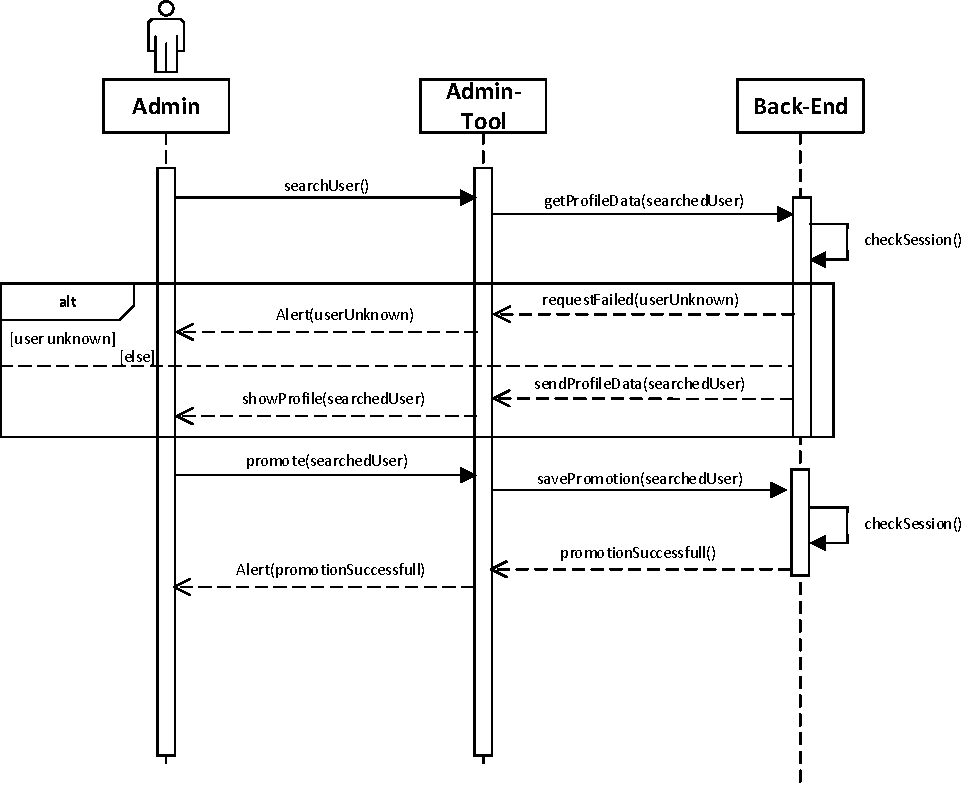
\includegraphics[width=0.9\textwidth]{figures/sequenz_F190.pdf}
\caption{Sequenzdiagramm zum Befördern eines Users}
\label{sequence_f190}
\end{figure}
Abbildung \ref{sequence_f190} beschreibt das Befördern eines Benutzers.

Zuerst wird für den Admin die Userdatenbank angezeigt. Hier kann er entweder manuell oder per Suchfunktion nach einem User suchen und diesen per Knopfdruck befördern, was dann im Back-End in den jeweiligen Userdaten registriert und gespeichert wird. 

Der Ablauf, einem User Adminrechte (<F200>) zu geben, gleicht dem des User Bef\"orderns.
%==================================================================

\newpage
\section{Analyse von Funktionalität <F210>: <Eine Trivia-Aufgabe erstellen>}
\begin{figure}[h]
\centering
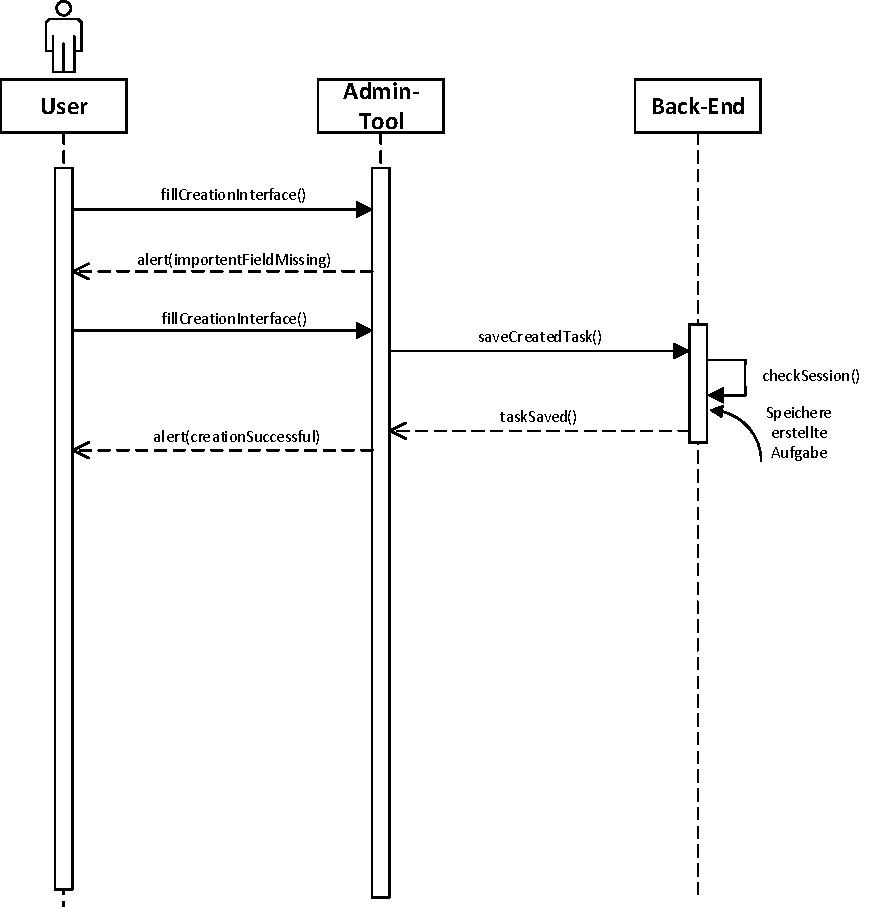
\includegraphics[width=0.9\textwidth]{figures/sequenz_F210.pdf}
\caption{Sequenzdiagramm für das Erstellen von Aufgaben}
\label{sequence_f210}
\end{figure}
Abbildung \ref{sequence_f210} beschreibt das Erstellen von eigenen Aufgaben.

Beförderte Nutzer können selber Aufgaben erstellen, welche später im Trivia Mode verwendet werden können.
Dafür steht im Admin-Tool ein Interface zur Verfügung, in das ganz einfach alle zur Aufgabe gehörigen Daten eingetragen und dann an das Back-End gesendet werden, wo die Aufgabe gespeichert wird. Sind nicht alle wichtigen Felder ausgefüllt, wird der User alarmiert und muss dies berichtigen, damit die Aufgabe abgespeichert werden kann.
%==================================================================

\newpage
\section{Analyse von Funktionalität <F220>: <Benutzeraufgaben bewerten>}
\begin{figure}[h]
\centering
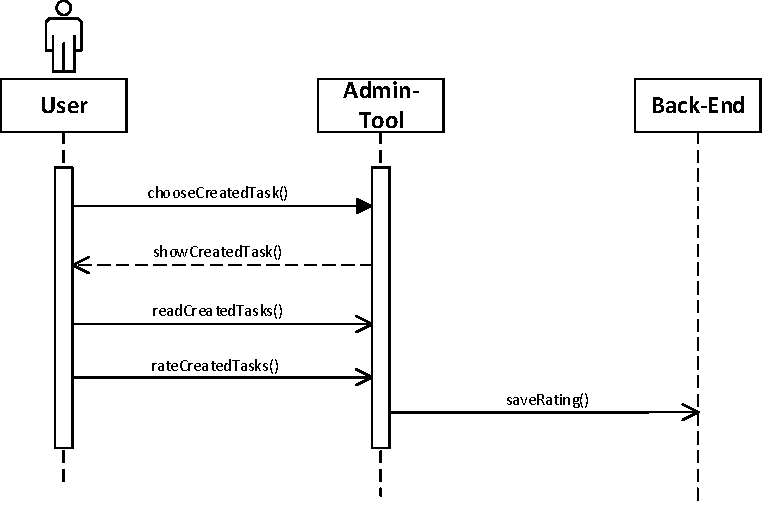
\includegraphics[width=0.9
\textwidth]{figures/sequenz_F220.pdf}
\caption{Sequenzdiagramm zum bewerten User-erstellter Aufgaben.}
\label{sequence_f220}
\end{figure}
Abbildung \ref{sequence_f220} zeigt den Ablauf, wie man eine von Usern erstellte Aufgabe bewertet.

In der Liste aller von Usern erstellten Aufgaben kann sich der User Aufgaben aussuchen, diese ansehen, sie bewerten und kommentieren. Die Bewertung wird dann im Back-End für die Aufgabe registriert und gespeichert. 
%==================================================================

\newpage
\section{Analyse von Funktionalität <F230>: <Hausaufgaben erstellen>}

Die Erstellung von Hausaufgaben gleicht der userseitigen Erstellung von Aufgaben, ist jedoch nur Administratoren zugänglich.

Der Unterschied zur normalen Aufgabenerstellung besteht darin, dass ein Aufgabenpaket erstellt wird. Dabei kann man entweder Aufgaben für das Paket neu erstellen, oder auf schon einmal erstellte Aufgaben, die in der Datenbank gespeichert sind, zugreifen. Diese Aufgabenpakete können dann noch mit zusätzlichen Parametern versehen werden, wie zum Beispiel einem Bearbeitungszeitraum oder einer Anzahl an Versuchen. 
